\chapter{Дарақтағы сұратымдар}

\index{дарақтағы сұратымдар}

Бұл тарауда түбірлі дарақтағы жолдар мен ішдарақтардағы 
сұратымдарды өңдейтін әдістер талқыланады.
Мысалы, оларға мынадай сұратымдар жатады:
% This chapter discusses techniques for
% processing queries on
% subtrees and paths of a rooted tree.
% For example, such queries are:

\begin{itemize}
\item төбенің $k$-бабасы қай төбе?
\item төбенің ішдарағындағы мәндер қосындысы неге тең?
\item екі төбе арасындағы жол мәндерінің қосындысы неге тең?
\item екі төбенің жақын арадағы ата-тегі қай төбе?
\end{itemize}

% \begin{itemize}
% \item what is the $k$th ancestor of a node?
% \item what is the sum of values in the subtree of a node?
% \item what is the sum of values on a path between two nodes?
% \item what is the lowest common ancestor of two nodes?
% \end{itemize}

\section{Бабалардың ізденісі}

\index{баба}

Түбірлі дарақта $x$ төбесінің $k$-бабасы дегеніміз $x$-төбеден
$k$ қадам жоғарыға жүретін жолда кездесетін төбе.
$\texttt{ancestor}(x,k)$ деп біз $x$-төбенің $k$-бабасын белгілейік
(немесе сәйкес бабасы болмаған жағдайда $0$ дейік).
Мысалы, келесі дарақта 
$\texttt{ancestor}(2,1)=1$ және $\texttt{ancestor}(8,2)=4$.
% The $k$th \key{ancestor} of a node $x$ in a rooted tree
% is the node that we will reach if we move $k$
% levels up from $x$.
% Let $\texttt{ancestor}(x,k)$ denote the $k$th ancestor of a node $x$
% (or $0$ if there is no such an ancestor).
% For example, in the following tree,
% $\texttt{ancestor}(2,1)=1$ and $\texttt{ancestor}(8,2)=4$.
\begin{center}
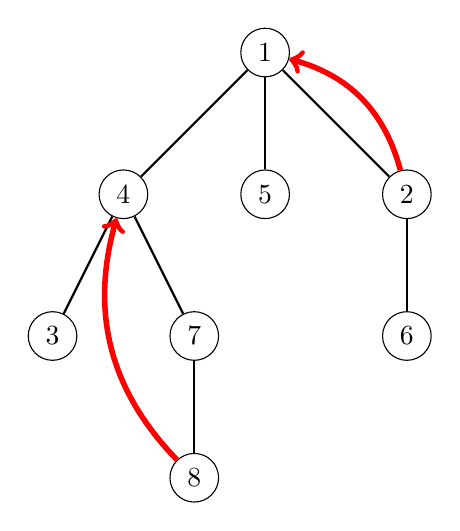
\begin{tikzpicture}[scale=0.9]
\node[draw, circle] (1) at (0,3) {$1$};
\node[draw, circle] (2) at (2,1) {$2$};
\node[draw, circle] (3) at (-2,1) {$4$};
\node[draw, circle] (4) at (0,1) {$5$};
\node[draw, circle] (5) at (2,-1) {$6$};
\node[draw, circle] (6) at (-3,-1) {$3$};
\node[draw, circle] (7) at (-1,-1) {$7$};
\node[draw, circle] (8) at (-1,-3) {$8$};
\path[draw,thick,-] (1) -- (2);
\path[draw,thick,-] (1) -- (3);
\path[draw,thick,-] (1) -- (4);
\path[draw,thick,-] (2) -- (5);
\path[draw,thick,-] (3) -- (6);
\path[draw,thick,-] (3) -- (7);
\path[draw,thick,-] (7) -- (8);

\path[draw=red,thick,->,line width=2pt] (8) edge [bend left] (3);
\path[draw=red,thick,->,line width=2pt] (2) edge [bend right] (1);
\end{tikzpicture}
\end{center}

Кез келген $\texttt{ancestor}(x,k)$ мәнін есептеудің оңай жолы -- 
дарақта $k$ рет үстіге қарай жүру.
Дегенмен, бұл әдістің уақытша күрделілігі $O(k)$ болғандықтан, баяу саналады.
Себебі $n$ төбесі бар графта төбелер бір тізбекте 
орналасуы мүмкін. Солайша, уақытша күрделілігі $O(n)$ болып кетуі ықтимал.

% An easy way to calculate any value of $\texttt{ancestor}(x,k)$
% is to perform a sequence of $k$ moves in the tree.
% However, the time complexity of this method
% is $O(k)$, which may be slow, because a tree of $n$
% nodes may have a chain of $n$ nodes.

Бақытымызға орай, 16.3 тарауында талқыланған әдіс арқылы 
кез келген $\texttt{ancestor}(x,k)$ мәнін алдын ала
өңдеуден кейін $O(\log k)$ уақыт ішінде табуға болады. 
Бұл жердегі идея $k$ саны екінің дәрежесі болатындай 
барлық $\texttt{ancestor}(x,k)$ мәндерін есептеп шығуға негізделеді.
Мысалы, жоғарыдағы дараққа келесі мәндер берілген:
% Fortunately, using a technique similar to that
% used in Chapter 16.3, any value of $\texttt{ancestor}(x,k)$
% can be efficiently calculated in $O(\log k)$ time
% after preprocessing.
% The idea is to precalculate all values $\texttt{ancestor}(x,k)$
% where $k \le n$ is a power of two.
% For example, the values for the above tree
% are as follows:

\begin{center}
\begin{tabular}{r|rrrrrrrrr}
$x$ & 1 & 2 & 3 & 4 & 5 & 6 & 7 & 8 \\
\hline
$\texttt{ancestor}(x,1)$ & 0 & 1 & 4 & 1 & 1 & 2 & 4 & 7 \\
$\texttt{ancestor}(x,2)$ & 0 & 0 & 1 & 0 & 0 & 1 & 1 & 4 \\
$\texttt{ancestor}(x,4)$ & 0 & 0 & 0 & 0 & 0 & 0 & 0 & 0 \\
$\cdots$ \\
\end{tabular}
\end{center}

Әр төбе үшін $O(\log n)$ мән есептелгендіктен, алдын ала өңдеу $O(n \log n)$ уақыт алады.
Бұдан соң $\texttt{ancestor}(x,k)$-ның кез келген мәнін
$k$-ның екі дәрежелі қосындыларына жіктеу арқылы табуға болады.
% The preprocessing takes $O(n \log n)$ time,
% because $O(\log n)$ values are calculated for each node.
% After this, any value of $\texttt{ancestor}(x,k)$ can be calculated
% in $O(\log k)$ time by representing $k$
% as a sum where each term is a power of two.

\section{Ішдарақтар және жолдар}

\index{дарақ айналымының жиымы}

\key{Дарақ айналымының жиымы}
түбірлі дарақтың төбелерін 
тереңдігі бойынша ізденіс арқылы жүру реттілігінде сақтайды.
Мысалға төмендегі дарақты алайық:
% A \key{tree traversal array} contains the nodes of a rooted tree
% in the order in which a depth-first search
% from the root node visits them.
% For example, in the tree
\begin{center}
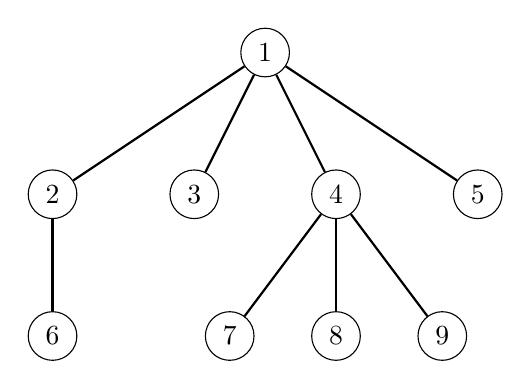
\begin{tikzpicture}[scale=0.9]
\node[draw, circle] (1) at (0,3) {$1$};
\node[draw, circle] (2) at (-3,1) {$2$};
\node[draw, circle] (3) at (-1,1) {$3$};
\node[draw, circle] (4) at (1,1) {$4$};
\node[draw, circle] (5) at (3,1) {$5$};
\node[draw, circle] (6) at (-3,-1) {$6$};
\node[draw, circle] (7) at (-0.5,-1) {$7$};
\node[draw, circle] (8) at (1,-1) {$8$};
\node[draw, circle] (9) at (2.5,-1) {$9$};

\path[draw,thick,-] (1) -- (2);
\path[draw,thick,-] (1) -- (3);
\path[draw,thick,-] (1) -- (4);
\path[draw,thick,-] (1) -- (5);
\path[draw,thick,-] (2) -- (6);
\path[draw,thick,-] (4) -- (7);
\path[draw,thick,-] (4) -- (8);
\path[draw,thick,-] (4) -- (9);
\end{tikzpicture}
\end{center}
тереңдігі бойынша ізденіс келесі ретпен жасалады:
% a depth-first search proceeds as follows:
\begin{center}
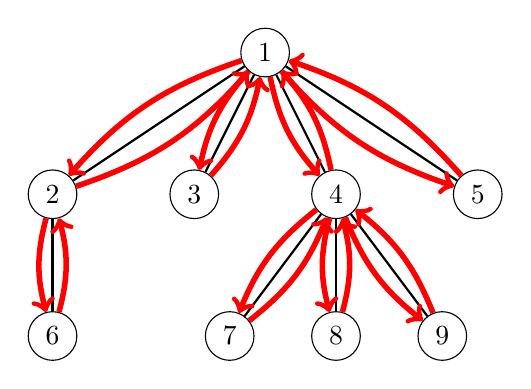
\begin{tikzpicture}[scale=0.9]
\node[draw, circle] (1) at (0,3) {$1$};
\node[draw, circle] (2) at (-3,1) {$2$};
\node[draw, circle] (3) at (-1,1) {$3$};
\node[draw, circle] (4) at (1,1) {$4$};
\node[draw, circle] (5) at (3,1) {$5$};
\node[draw, circle] (6) at (-3,-1) {$6$};
\node[draw, circle] (7) at (-0.5,-1) {$7$};
\node[draw, circle] (8) at (1,-1) {$8$};
\node[draw, circle] (9) at (2.5,-1) {$9$};

\path[draw,thick,-] (1) -- (2);
\path[draw,thick,-] (1) -- (3);
\path[draw,thick,-] (1) -- (4);
\path[draw,thick,-] (1) -- (5);
\path[draw,thick,-] (2) -- (6);
\path[draw,thick,-] (4) -- (7);
\path[draw,thick,-] (4) -- (8);
\path[draw,thick,-] (4) -- (9);


\path[draw=red,thick,->,line width=2pt] (1) edge [bend right=15] (2);
\path[draw=red,thick,->,line width=2pt] (2) edge [bend right=15] (6);
\path[draw=red,thick,->,line width=2pt] (6) edge [bend right=15] (2);
\path[draw=red,thick,->,line width=2pt] (2) edge [bend right=15] (1);
\path[draw=red,thick,->,line width=2pt] (1) edge [bend right=15] (3);
\path[draw=red,thick,->,line width=2pt] (3) edge [bend right=15] (1);
\path[draw=red,thick,->,line width=2pt] (1) edge [bend right=15] (4);
\path[draw=red,thick,->,line width=2pt] (4) edge [bend right=15] (7);
\path[draw=red,thick,->,line width=2pt] (7) edge [bend right=15] (4);
\path[draw=red,thick,->,line width=2pt] (4) edge [bend right=15] (8);
\path[draw=red,thick,->,line width=2pt] (8) edge [bend right=15] (4);
\path[draw=red,thick,->,line width=2pt] (4) edge [bend right=15] (9);
\path[draw=red,thick,->,line width=2pt] (9) edge [bend right=15] (4);
\path[draw=red,thick,->,line width=2pt] (4) edge [bend right=15] (1);
\path[draw=red,thick,->,line width=2pt] (1) edge [bend right=15] (5);
\path[draw=red,thick,->,line width=2pt] (5) edge [bend right=15] (1);

\end{tikzpicture}
\end{center}
Сол себепті дарақ айналымының жиымы төмендегідей болмақ:
% Hence, the corresponding tree traversal array is as follows:
\begin{center}
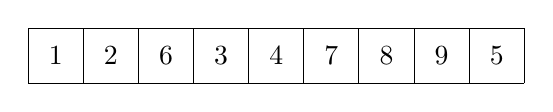
\begin{tikzpicture}[scale=0.7]
\draw (0,0) grid (9,1);

\node at (0.5,0.5) {$1$};
\node at (1.5,0.5) {$2$};
\node at (2.5,0.5) {$6$};
\node at (3.5,0.5) {$3$};
\node at (4.5,0.5) {$4$};
\node at (5.5,0.5) {$7$};
\node at (6.5,0.5) {$8$};
\node at (7.5,0.5) {$9$};
\node at (8.5,0.5) {$5$};
% 
% \footnotesize
% \node at (0.5,1.4) {$1$};
% \node at (1.5,1.4) {$2$};
% \node at (2.5,1.4) {$3$};
% \node at (3.5,1.4) {$4$};
% \node at (4.5,1.4) {$5$};
% \node at (5.5,1.4) {$6$};
% \node at (6.5,1.4) {$7$};
% \node at (7.5,1.4) {$8$};
% \node at (8.5,1.4) {$9$};
\end{tikzpicture}
\end{center}

\subsubsection{Ішдарақ сұратымдары}

Дарақтың әр ішдарағы дарақ айналымының жиымындағы бір ішжиымға сәйкес келеді.
Бұл ішжиымдағы бірінші элемент -- ішдарақтың түбірі.
Мысалы, келесі ішдарақ $4$-төбе ішдарағының 
төбелерін қамтиды:
% Each subtree of a tree corresponds to a subarray
% of the tree traversal array such that
% the first element of the subarray is the root node.
% For example, the following subarray contains the
% nodes of the subtree of node $4$:
\begin{center}
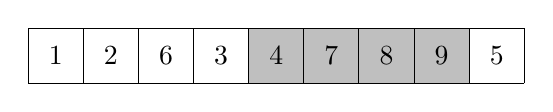
\begin{tikzpicture}[scale=0.7]
\fill[color=lightgray] (4,0) rectangle (8,1);
\draw (0,0) grid (9,1);

\node at (0.5,0.5) {$1$};
\node at (1.5,0.5) {$2$};
\node at (2.5,0.5) {$6$};
\node at (3.5,0.5) {$3$};
\node at (4.5,0.5) {$4$};
\node at (5.5,0.5) {$7$};
\node at (6.5,0.5) {$8$};
\node at (7.5,0.5) {$9$};
\node at (8.5,0.5) {$5$};
% 
% \footnotesize
% \node at (0.5,1.4) {$1$};
% \node at (1.5,1.4) {$2$};
% \node at (2.5,1.4) {$3$};
% \node at (3.5,1.4) {$4$};
% \node at (4.5,1.4) {$5$};
% \node at (5.5,1.4) {$6$};
% \node at (6.5,1.4) {$7$};
% \node at (7.5,1.4) {$8$};
% \node at (8.5,1.4) {$9$};
\end{tikzpicture}
\end{center}
Осы дерек арқылы біз ішдараққа байланысты сұратымдарды
тиімді өңдей аламыз.
Мысалы, әр төбе үшін бір сан бекітілген есепті қарастырайық.
Бұл есепте біз келесі сұратымдармен жұмыс жасаймыз:
% Using this fact, we can efficiently process queries
% that are related to subtrees of a tree.
% As an example, consider a problem where each node
% is assigned a value, and our task is to support
% the following queries:
\begin{itemize}
\item төбедегі санды басқа санмен жаңарту
\item төбенің ішдарағындағы мәндер қосындысын есептеу
\end{itemize}
% \begin{itemize}
% \item update the value of a node
% \item calculate the sum of values in the subtree of a node
% \end{itemize}

Көк сандармен төбелердің мәндері берілген дарақты 
қарастырайық.
Мысалы, $4$-төбе үшін ішдарағының қосындысы -- $3+4+3+1=11$.
% Consider the following tree where the blue numbers
% are the values of the nodes.
% For example, the sum of the subtree of node $4$
% is $3+4+3+1=11$.

\begin{center}
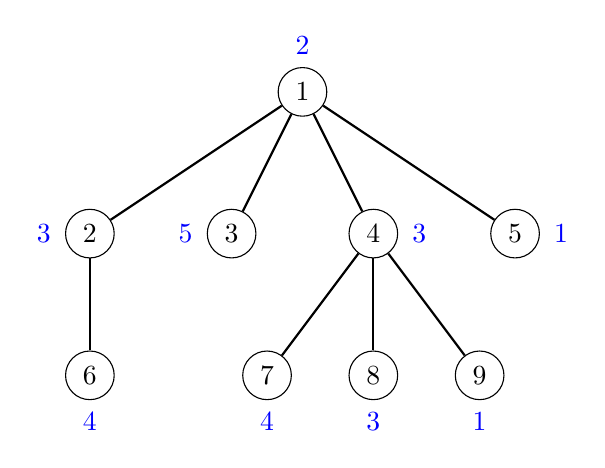
\begin{tikzpicture}[scale=0.9]
\node[draw, circle] (1) at (0,3) {$1$};
\node[draw, circle] (2) at (-3,1) {$2$};
\node[draw, circle] (3) at (-1,1) {$3$};
\node[draw, circle] (4) at (1,1) {$4$};
\node[draw, circle] (5) at (3,1) {$5$};
\node[draw, circle] (6) at (-3,-1) {$6$};
\node[draw, circle] (7) at (-0.5,-1) {$7$};
\node[draw, circle] (8) at (1,-1) {$8$};
\node[draw, circle] (9) at (2.5,-1) {$9$};

\path[draw,thick,-] (1) -- (2);
\path[draw,thick,-] (1) -- (3);
\path[draw,thick,-] (1) -- (4);
\path[draw,thick,-] (1) -- (5);
\path[draw,thick,-] (2) -- (6);
\path[draw,thick,-] (4) -- (7);
\path[draw,thick,-] (4) -- (8);
\path[draw,thick,-] (4) -- (9);

\node[color=blue] at (0,3+0.65) {2};
\node[color=blue] at (-3-0.65,1) {3};
\node[color=blue] at (-1-0.65,1) {5};
\node[color=blue] at (1+0.65,1) {3};
\node[color=blue] at (3+0.65,1) {1};
\node[color=blue] at (-3,-1-0.65) {4};
\node[color=blue] at (-0.5,-1-0.65) {4};
\node[color=blue] at (1,-1-0.65) {3};
\node[color=blue] at (2.5,-1-0.65) {1};
\end{tikzpicture}
\end{center}

Бұл есепті шығару үшін біз әр төбе үшін оның идентификаторы, ішдарағының өлшемі мен оның мәні сақталатын  дарақ айналымының жиымын құрамыз.
Мысалы, жоғарыда келтірілген дарақтың жиымы келісідей болмақ:
% The idea is to construct a tree traversal array that contains
% three values for each node: the identifier of the node,
% the size of the subtree, and the value of the node.
% For example, the array for the above tree is as follows:

\begin{center}
\begin{tikzpicture}[scale=0.7]
\draw (0,1) grid (9,-2);

\node[left] at (-1,0.5) {төбе идентификаторы};
\node[left] at (-1,-0.5) {ішдарақтың өлшемі};
\node[left] at (-1,-1.5) {төбенің мәні};

\node at (0.5,0.5) {$1$};
\node at (1.5,0.5) {$2$};
\node at (2.5,0.5) {$6$};
\node at (3.5,0.5) {$3$};
\node at (4.5,0.5) {$4$};
\node at (5.5,0.5) {$7$};
\node at (6.5,0.5) {$8$};
\node at (7.5,0.5) {$9$};
\node at (8.5,0.5) {$5$};

\node at (0.5,-0.5) {$9$};
\node at (1.5,-0.5) {$2$};
\node at (2.5,-0.5) {$1$};
\node at (3.5,-0.5) {$1$};
\node at (4.5,-0.5) {$4$};
\node at (5.5,-0.5) {$1$};
\node at (6.5,-0.5) {$1$};
\node at (7.5,-0.5) {$1$};
\node at (8.5,-0.5) {$1$};

\node at (0.5,-1.5) {$2$};
\node at (1.5,-1.5) {$3$};
\node at (2.5,-1.5) {$4$};
\node at (3.5,-1.5) {$5$};
\node at (4.5,-1.5) {$3$};
\node at (5.5,-1.5) {$4$};
\node at (6.5,-1.5) {$3$};
\node at (7.5,-1.5) {$1$};
\node at (8.5,-1.5) {$1$};
% 
% \footnotesize
% \node at (0.5,1.4) {$1$};
% \node at (1.5,1.4) {$2$};
% \node at (2.5,1.4) {$3$};
% \node at (3.5,1.4) {$4$};
% \node at (4.5,1.4) {$5$};
% \node at (5.5,1.4) {$6$};
% \node at (6.5,1.4) {$7$};
% \node at (7.5,1.4) {$8$};
% \node at (8.5,1.4) {$9$};
\end{tikzpicture}
\end{center}

Бұл жиымды қолдана отырып, кез келген ішдарақтың 
қосындысын алдымен ішдарақтың өлшемін, кейін ішдараққа сәйкес төбелердің
мәндерін табу арқылы есептей аламыз.
Мысалы, $4$-төбе ішдарағының қосындысын осылай табуға болады:
% Using this array, we can calculate the sum of values
% in any subtree by first finding out the size of the subtree
% and then the values of the corresponding nodes.
% For example, the values in the subtree of node $4$
% can be found as follows:

\begin{center}
\begin{tikzpicture}[scale=0.7]
\fill[color=lightgray] (4,1) rectangle (5,0);
\fill[color=lightgray] (4,0) rectangle (5,-1);
\fill[color=lightgray] (4,-1) rectangle (8,-2);
\draw (0,1) grid (9,-2);

\node[left] at (-1,0.5) {төбе идентификаторы};
\node[left] at (-1,-0.5) {ішдарақтың өлшемі};
\node[left] at (-1,-1.5) {төбенің мәні};

\node at (0.5,0.5) {$1$};
\node at (1.5,0.5) {$2$};
\node at (2.5,0.5) {$6$};
\node at (3.5,0.5) {$3$};
\node at (4.5,0.5) {$4$};
\node at (5.5,0.5) {$7$};
\node at (6.5,0.5) {$8$};
\node at (7.5,0.5) {$9$};
\node at (8.5,0.5) {$5$};

\node at (0.5,-0.5) {$9$};
\node at (1.5,-0.5) {$2$};
\node at (2.5,-0.5) {$1$};
\node at (3.5,-0.5) {$1$};
\node at (4.5,-0.5) {$4$};
\node at (5.5,-0.5) {$1$};
\node at (6.5,-0.5) {$1$};
\node at (7.5,-0.5) {$1$};
\node at (8.5,-0.5) {$1$};

\node at (0.5,-1.5) {$2$};
\node at (1.5,-1.5) {$3$};
\node at (2.5,-1.5) {$4$};
\node at (3.5,-1.5) {$5$};
\node at (4.5,-1.5) {$3$};
\node at (5.5,-1.5) {$4$};
\node at (6.5,-1.5) {$3$};
\node at (7.5,-1.5) {$1$};
\node at (8.5,-1.5) {$1$};
% 
% \footnotesize
% \node at (0.5,1.4) {$1$};
% \node at (1.5,1.4) {$2$};
% \node at (2.5,1.4) {$3$};
% \node at (3.5,1.4) {$4$};
% \node at (4.5,1.4) {$5$};
% \node at (5.5,1.4) {$6$};
% \node at (6.5,1.4) {$7$};
% \node at (7.5,1.4) {$8$};
% \node at (8.5,1.4) {$9$};
\end{tikzpicture}
\end{center}

Сұратымдарға оңтайлы жауап беру үшін төбелердің мәнін бинарлы индекстелген дарақта немесе 
кесінділер дарағында сақтасақ, жеткілікті.
Содан кейін біз мәндерді жаңартуды да, мәндердің қосындысын есептеуді де $O(\log n)$ уақытта жүзеге асыра аламыз. 
% To answer the queries efficiently,
% it suffices to store the values of the
% nodes in a binary indexed or segment tree.
% After this, we can both update a value
% and calculate the sum of values in $O(\log n)$ time.

\subsubsection{Жол сұратымдары}

Дарақ айналымының жиымын қолдану арқылы түбірден дарақтағы
кез келген төбеге дейінгі жолдағы мәндердің
қосындысын тиімді есептей аламыз.
Келесі сұратымдарды қолдайтын есепті қарастырайық:
% Using a tree traversal array, we can also efficiently
% calculate sums of values on
% paths from the root node to any
% node of the tree.
% Consider a problem where our task
% is to support the following queries:
\begin{itemize}
\item төбедегі мәнді ауыстыру
\item кез келген төбеден түбірге дейінгі мәндердің қосындысын 
есептеп шығу
\end{itemize}

Мысалы, төменде көрсетілген дарақтағы $7$-төбеден түбірге дейінгі мәндердің 
қосындысы -- $4+5+5=14$:
% For example, in the following tree,
% the sum of values from the root node to node 7 is
% $4+5+5=14$:

\begin{center}
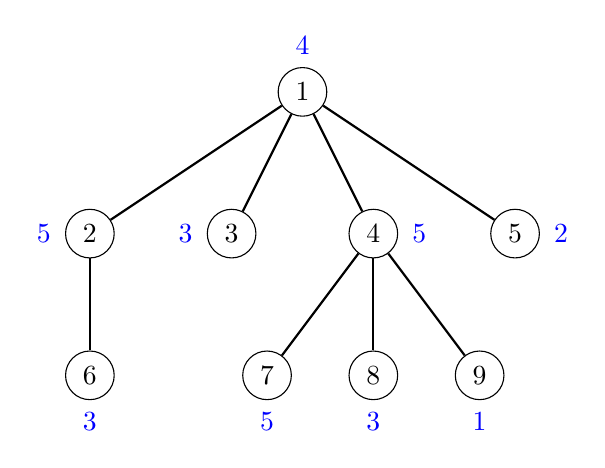
\begin{tikzpicture}[scale=0.9]
\node[draw, circle] (1) at (0,3) {$1$};
\node[draw, circle] (2) at (-3,1) {$2$};
\node[draw, circle] (3) at (-1,1) {$3$};
\node[draw, circle] (4) at (1,1) {$4$};
\node[draw, circle] (5) at (3,1) {$5$};
\node[draw, circle] (6) at (-3,-1) {$6$};
\node[draw, circle] (7) at (-0.5,-1) {$7$};
\node[draw, circle] (8) at (1,-1) {$8$};
\node[draw, circle] (9) at (2.5,-1) {$9$};

\path[draw,thick,-] (1) -- (2);
\path[draw,thick,-] (1) -- (3);
\path[draw,thick,-] (1) -- (4);
\path[draw,thick,-] (1) -- (5);
\path[draw,thick,-] (2) -- (6);
\path[draw,thick,-] (4) -- (7);
\path[draw,thick,-] (4) -- (8);
\path[draw,thick,-] (4) -- (9);

\node[color=blue] at (0,3+0.65) {4};
\node[color=blue] at (-3-0.65,1) {5};
\node[color=blue] at (-1-0.65,1) {3};
\node[color=blue] at (1+0.65,1) {5};
\node[color=blue] at (3+0.65,1) {2};
\node[color=blue] at (-3,-1-0.65) {3};
\node[color=blue] at (-0.5,-1-0.65) {5};
\node[color=blue] at (1,-1-0.65) {3};
\node[color=blue] at (2.5,-1-0.65) {1};
\end{tikzpicture}
\end{center}

Біз бұл есепті бұрынғыдай шеше аламыз. Бірақ 
жиымның соңғы жолындағы мәндер енді түбірден сол төбеге дейінгі жол қосындысына тең болады.
Мысалы, келесі жиым жоғарыда келтірілген дараққа сәйкес келеді:
% We can solve this problem like before,
% but now each value in the last row of the array is the sum of values
% on a path from the root to the node.
% For example, the following array corresponds to the above tree:
\begin{center}
\begin{tikzpicture}[scale=0.7]
\draw (0,1) grid (9,-2);

\node[left] at (-1,0.5) {төбе идентификаторы};
\node[left] at (-1,-0.5) {ішдарақтың өлшемі};
\node[left] at (-1,-1.5) {жол қосындысы};

\node at (0.5,0.5) {$1$};
\node at (1.5,0.5) {$2$};
\node at (2.5,0.5) {$6$};
\node at (3.5,0.5) {$3$};
\node at (4.5,0.5) {$4$};
\node at (5.5,0.5) {$7$};
\node at (6.5,0.5) {$8$};
\node at (7.5,0.5) {$9$};
\node at (8.5,0.5) {$5$};

\node at (0.5,-0.5) {$9$};
\node at (1.5,-0.5) {$2$};
\node at (2.5,-0.5) {$1$};
\node at (3.5,-0.5) {$1$};
\node at (4.5,-0.5) {$4$};
\node at (5.5,-0.5) {$1$};
\node at (6.5,-0.5) {$1$};
\node at (7.5,-0.5) {$1$};
\node at (8.5,-0.5) {$1$};

\node at (0.5,-1.5) {$4$};
\node at (1.5,-1.5) {$9$};
\node at (2.5,-1.5) {$12$};
\node at (3.5,-1.5) {$7$};
\node at (4.5,-1.5) {$9$};
\node at (5.5,-1.5) {$14$};
\node at (6.5,-1.5) {$12$};
\node at (7.5,-1.5) {$10$};
\node at (8.5,-1.5) {$6$};
\end{tikzpicture}
\end{center}

Егер төбедегі мән $x$-ке артса, ішдарақтағы барлық төбелердің
қосындылары да $x$-ке артады.
Мысалы, егер $4$-төбенің мәнін $1$-ге арттырсақ,  
жиым төмендегідей болып өзгереді:
% When the value of a node increases by $x$,
% the sums of all nodes in its subtree increase by $x$.
% For example, if the value of node 4 increases by 1,
% the array changes as follows:

\begin{center}
\begin{tikzpicture}[scale=0.7]
\fill[color=lightgray] (4,-1) rectangle (8,-2);
\draw (0,1) grid (9,-2);

\node[left] at (-1,0.5) {төбе идентификаторы};
\node[left] at (-1,-0.5) {ішдарақтың өлшемі};
\node[left] at (-1,-1.5) {жол қосындысы};

\node at (0.5,0.5) {$1$};
\node at (1.5,0.5) {$2$};
\node at (2.5,0.5) {$6$};
\node at (3.5,0.5) {$3$};
\node at (4.5,0.5) {$4$};
\node at (5.5,0.5) {$7$};
\node at (6.5,0.5) {$8$};
\node at (7.5,0.5) {$9$};
\node at (8.5,0.5) {$5$};

\node at (0.5,-0.5) {$9$};
\node at (1.5,-0.5) {$2$};
\node at (2.5,-0.5) {$1$};
\node at (3.5,-0.5) {$1$};
\node at (4.5,-0.5) {$4$};
\node at (5.5,-0.5) {$1$};
\node at (6.5,-0.5) {$1$};
\node at (7.5,-0.5) {$1$};
\node at (8.5,-0.5) {$1$};

\node at (0.5,-1.5) {$4$};
\node at (1.5,-1.5) {$9$};
\node at (2.5,-1.5) {$12$};
\node at (3.5,-1.5) {$7$};
\node at (4.5,-1.5) {$10$};
\node at (5.5,-1.5) {$15$};
\node at (6.5,-1.5) {$13$};
\node at (7.5,-1.5) {$11$};
\node at (8.5,-1.5) {$6$};
\end{tikzpicture}
\end{center}

Екі операцияны да қолдау үшін біз диапазондағы 
барлық мәндерді арттыра отырып, бір мән алуымыз қажет.
Мұны бинарлы индекстелген дарақты немесе кесінділер дарағын қолдану
арқылы $O(\log n)$ уақыт ішінде іске асыра аламыз.
% Thus, to support both the operations,
% we should be able to increase all values
% in a range and retrieve a single value.
% This can be done in $O(\log n)$ time
% using a binary indexed
% or segment tree (see Chapter 9.4).

\section{Жақын арадағы ата-тек}

\index{жақын арадағы ата-тек}

Екі төбенің жақын арадағы ата-тегі дегеніміз
ішдарағы екі төбені де қамтитын ең төмен орналасқан төбе.
Екі төбенің жақын арадағы ата-тегін тиімді 
табуға арналған есептер жиі кездеседі.
% The \key{lowest common ancestor}
% of two nodes of a rooted tree is the lowest node
% whose subtree contains both the nodes.
% A typical problem is to efficiently process
% queries that ask to find the lowest
% common ancestor of two nodes.

Мысалы, келесі дарақтағы 5 және 8 төбелерінің 
жақын арадағы ата-тегі -- 2-төбе:
% For example, in the following tree,
% the lowest common ancestor of nodes 5 and 8
% is node 2:
\begin{center}
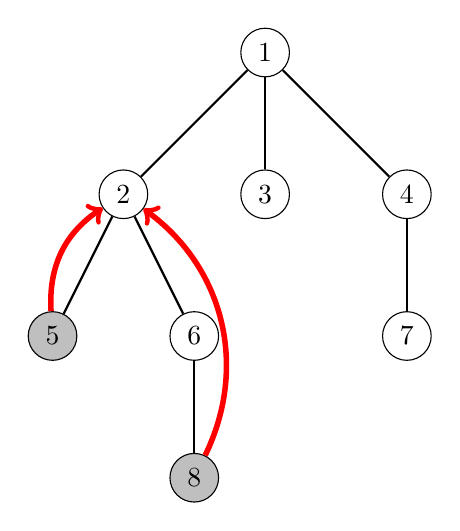
\begin{tikzpicture}[scale=0.9]
\node[draw, circle] (1) at (0,3) {$1$};
\node[draw, circle] (2) at (2,1) {$4$};
\node[draw, circle] (3) at (-2,1) {$2$};
\node[draw, circle] (4) at (0,1) {$3$};
\node[draw, circle] (5) at (2,-1) {$7$};
\node[draw, circle, fill=lightgray] (6) at (-3,-1) {$5$};
\node[draw, circle] (7) at (-1,-1) {$6$};
\node[draw, circle, fill=lightgray] (8) at (-1,-3) {$8$};
\path[draw,thick,-] (1) -- (2);
\path[draw,thick,-] (1) -- (3);
\path[draw,thick,-] (1) -- (4);
\path[draw,thick,-] (2) -- (5);
\path[draw,thick,-] (3) -- (6);
\path[draw,thick,-] (3) -- (7);
\path[draw,thick,-] (7) -- (8);

\path[draw=red,thick,->,line width=2pt] (6) edge [bend left] (3);
\path[draw=red,thick,->,line width=2pt] (8) edge [bend right=40] (3);
\end{tikzpicture}
\end{center}

Енді біз жақын арадағы ата-текті табуға көмектесетін
екі тиімді әдісті талқылаймыз.
% Next we will discuss two efficient techniques for
% finding the lowest common ancestor of two nodes.

\subsubsection{1-әдіс}

Біз бұған дейін дарақтағы кез келген төбенің 
$k$-бабасын табудың тиімді жолдарын қарастырдық. 
Осы әдісті қолдана отырып, жақын арадағы ата-текті табу
есебін де екі бөлікке бөлуге болады:
% One way to solve the problem is to use the fact
% that we can efficiently find the $k$th
% ancestor of any node in the tree.
% Using this, we can divide the problem of
% finding the lowest common ancestor into two parts.

Есепті шығару барысында біз  екі нұсқағышты қолданамыз. Бұл екі нұсқағыш басынан-ақ біз табуға тиісті  
жақын арадағы ата-текке қарай бағытталады.
Алдымен нұсқағыштар бағытталған төбелердің бір деңгейде орналасқанын тексеріп аламыз. 
Егер олай болмаса, нұсқағыштардың біреуін жоғарыға жылжытамыз.
% We use two pointers that initially point to the
% two nodes whose lowest common ancestor we should find.
% First, we move one of the pointers upwards
% so that both pointers point to nodes at the same level.

Үлгідегі дарақта біз $8$-төбеде тұрған нұсқағышты бір деңгей 
жоғарыға көтереміз. Осылайша ол $6$-төбеге жетіп, екі нұсқағыш та бір деңгейде болады.
% In the example scenario, we move the second pointer one
% level up so that it points to node 6
% which is at the same level with node 5:

\begin{center}
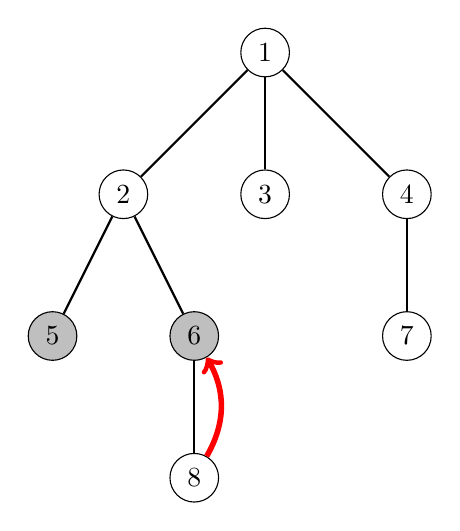
\begin{tikzpicture}[scale=0.9]
\node[draw, circle] (1) at (0,3) {$1$};
\node[draw, circle] (2) at (2,1) {$4$};
\node[draw, circle] (3) at (-2,1) {$2$};
\node[draw, circle] (4) at (0,1) {$3$};
\node[draw, circle] (5) at (2,-1) {$7$};
\node[draw, circle,fill=lightgray] (6) at (-3,-1) {$5$};
\node[draw, circle,fill=lightgray] (7) at (-1,-1) {$6$};
\node[draw, circle] (8) at (-1,-3) {$8$};
\path[draw,thick,-] (1) -- (2);
\path[draw,thick,-] (1) -- (3);
\path[draw,thick,-] (1) -- (4);
\path[draw,thick,-] (2) -- (5);
\path[draw,thick,-] (3) -- (6);
\path[draw,thick,-] (3) -- (7);
\path[draw,thick,-] (7) -- (8);

\path[draw=red,thick,->,line width=2pt] (8) edge [bend right] (7);
\end{tikzpicture}
\end{center}

Кейін біз екі нұсқағыш бір төбеде кездесетіндей
минималды қадам санын табамыз.
Осы төбе жақын арадағы ата-тегі болады.
% After this, we determine the minimum number of steps
% needed to move both pointers upwards so that
% they will point to the same node.
% The node to which the pointers point after this
% is the lowest common ancestor.

Мысалдағы графта нұсқағышты бір қадам жоғарыға
жылжыту жеткілікті болып тұр. Сонда олар $2$-төбеге нұсқайды. 
Бұл -- жақын арадағы ата-тек:
% In the example scenario, it suffices to move both pointers
% one step upwards to node 2,
% which is the lowest common ancestor:

\begin{center}
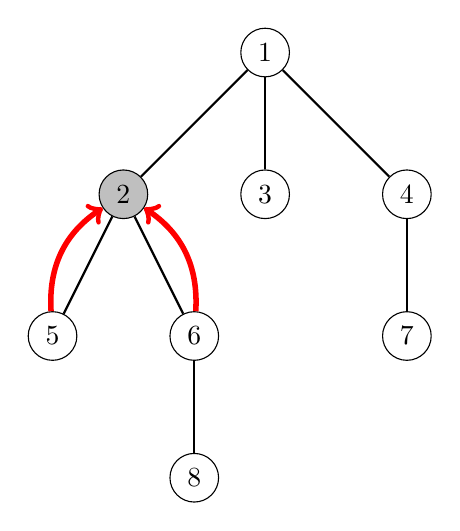
\begin{tikzpicture}[scale=0.9]
\node[draw, circle] (1) at (0,3) {$1$};
\node[draw, circle] (2) at (2,1) {$4$};
\node[draw, circle,fill=lightgray] (3) at (-2,1) {$2$};
\node[draw, circle] (4) at (0,1) {$3$};
\node[draw, circle] (5) at (2,-1) {$7$};
\node[draw, circle] (6) at (-3,-1) {$5$};
\node[draw, circle] (7) at (-1,-1) {$6$};
\node[draw, circle] (8) at (-1,-3) {$8$};
\path[draw,thick,-] (1) -- (2);
\path[draw,thick,-] (1) -- (3);
\path[draw,thick,-] (1) -- (4);
\path[draw,thick,-] (2) -- (5);
\path[draw,thick,-] (3) -- (6);
\path[draw,thick,-] (3) -- (7);
\path[draw,thick,-] (7) -- (8);

\path[draw=red,thick,->,line width=2pt] (6) edge [bend left] (3);
\path[draw=red,thick,->,line width=2pt] (7) edge [bend right] (3);
\end{tikzpicture}
\end{center}

Алгоритмнің екі бөлігінің де алдын ала өңделген
ақпаратты пайдаланып, $O(\log n)$ уақытында орындалуы 
мүмкін болғандықтан, жақын арадағы ата-тектерді $O(\log n)$ 
уақытында таба аламыз.
% Since both parts of the algorithm can be performed in
% $O(\log n)$ time using precomputed information,
% we can find the lowest common ancestor of any two
% nodes in $O(\log n)$ time.

\subsubsection{2-әдіс}

Осы есепті басқа жолмен, атап айтқанда дарақ айналымының жиымын 
қолдану арқылы да \footnote{Аталмыш жақын арадағы ата-текті табу алгоритмі осы жерде көрсетілген \cite{ben00}. Бұл әдіс кейде \index{Эйлер өту әдісі} (Euler tour technique) деп те аталады \cite{tar84}.} шығаруға болады.
Мұндағы идея тағы да тереңдігі бойынша ізденіс жасау арқылы төбелерді өтіп шығуға негізделеді.
% \key{Euler tour technique} \cite{tar84}.}.
% This technique is sometimes called the \index{Euler tour technique}
% \key{Euler tour technique} \cite{tar84}.}.
% Another way to solve the problem is based on
% a tree traversal array\footnote{This lowest common ancestor algorithm was presented in \cite{ben00}.
% This technique is sometimes called the \index{Euler tour technique}
% \key{Euler tour technique} \cite{tar84}.}.
% Once again, the idea is to traverse the nodes
% using a depth-first search:

\begin{center}
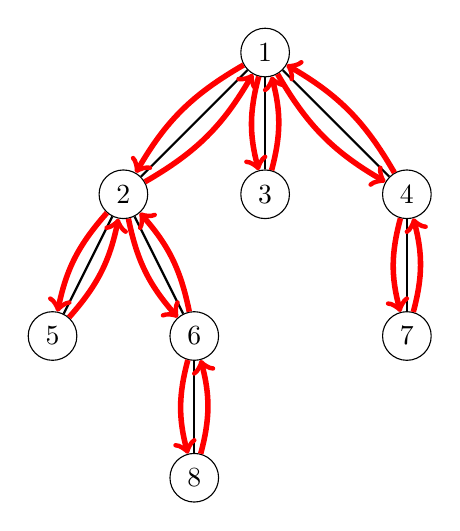
\begin{tikzpicture}[scale=0.9]
\node[draw, circle] (1) at (0,3) {$1$};
\node[draw, circle] (2) at (2,1) {$4$};
\node[draw, circle] (3) at (-2,1) {$2$};
\node[draw, circle] (4) at (0,1) {$3$};
\node[draw, circle] (5) at (2,-1) {$7$};
\node[draw, circle] (6) at (-3,-1) {$5$};
\node[draw, circle] (7) at (-1,-1) {$6$};
\node[draw, circle] (8) at (-1,-3) {$8$};
\path[draw,thick,-] (1) -- (2);
\path[draw,thick,-] (1) -- (3);
\path[draw,thick,-] (1) -- (4);
\path[draw,thick,-] (2) -- (5);
\path[draw,thick,-] (3) -- (6);
\path[draw,thick,-] (3) -- (7);
\path[draw,thick,-] (7) -- (8);

\path[draw=red,thick,->,line width=2pt] (1) edge [bend right=15] (3);
\path[draw=red,thick,->,line width=2pt] (3) edge [bend right=15] (6);
\path[draw=red,thick,->,line width=2pt] (6) edge [bend right=15] (3);
\path[draw=red,thick,->,line width=2pt] (3) edge [bend right=15] (7);
\path[draw=red,thick,->,line width=2pt] (7) edge [bend right=15] (8);
\path[draw=red,thick,->,line width=2pt] (8) edge [bend right=15] (7);
\path[draw=red,thick,->,line width=2pt] (7) edge [bend right=15] (3);
\path[draw=red,thick,->,line width=2pt] (3) edge [bend right=15] (1);
\path[draw=red,thick,->,line width=2pt] (1) edge [bend right=15] (4);
\path[draw=red,thick,->,line width=2pt] (4) edge [bend right=15] (1);
\path[draw=red,thick,->,line width=2pt] (1) edge [bend right=15] (2);
\path[draw=red,thick,->,line width=2pt] (2) edge [bend right=15] (5);
\path[draw=red,thick,->,line width=2pt] (5) edge [bend right=15] (2);
\path[draw=red,thick,->,line width=2pt] (2) edge [bend right=15] (1);
\end{tikzpicture}
\end{center}

Дегенмен, біз осыған дейін қарастырған жиымнан басқа жиымды
қолданамыз, төбені тек алғаш өткенде ғана емес, төбеден әр 
өткен сайын жиымға қосып отырамыз.
Демек, $k$ ұлдары бар төбе жиымда $k+1$ рет кездеседі және 
жиымда жалпы $2n-1$ төбе болады.
% However, we use a different tree
% traversal array than before:
% we add each node to the array \emph{always}
% when the depth-first search walks through the node,
% and not only at the first visit.
% Hence, a node that has $k$ children appears $k+1$ times
% in the array and there are a total of $2n-1$
% nodes in the array.

Біз жиымда екі мәнді сақтаймыз. Олар:
төбенің идентификаторы және төбенің дарақтағы тереңдігі.
Келесі жиым жоғарыдағы дараққа сәйкес келеді:
% We store two values in the array:
% the identifier of the node and the depth of the 
% node in the tree.
% The following array corresponds to the above tree:

\begin{center}
\begin{tikzpicture}[scale=0.7]

\node[left] at (-1,1.5) {төбе идентификаторы};
\node[left] at (-1,0.5) {тереңдігі};

\draw (0,1) grid (15,2);
\node at (0.5,1.5) {$1$};
\node at (1.5,1.5) {$2$};
\node at (2.5,1.5) {$5$};
\node at (3.5,1.5) {$2$};
\node at (4.5,1.5) {$6$};
\node at (5.5,1.5) {$8$};
\node at (6.5,1.5) {$6$};
\node at (7.5,1.5) {$2$};
\node at (8.5,1.5) {$1$};
\node at (9.5,1.5) {$3$};
\node at (10.5,1.5) {$1$};
\node at (11.5,1.5) {$4$};
\node at (12.5,1.5) {$7$};
\node at (13.5,1.5) {$4$};
\node at (14.5,1.5) {$1$};

\draw (0,0) grid (15,1);
\node at (0.5,0.5) {$1$};
\node at (1.5,0.5) {$2$};
\node at (2.5,0.5) {$3$};
\node at (3.5,0.5) {$2$};
\node at (4.5,0.5) {$3$};
\node at (5.5,0.5) {$4$};
\node at (6.5,0.5) {$3$};
\node at (7.5,0.5) {$2$};
\node at (8.5,0.5) {$1$};
\node at (9.5,0.5) {$2$};
\node at (10.5,0.5) {$1$};
\node at (11.5,0.5) {$2$};
\node at (12.5,0.5) {$3$};
\node at (13.5,0.5) {$2$};
\node at (14.5,0.5) {$1$};

\footnotesize
\node at (0.5,2.5) {$0$};
\node at (1.5,2.5) {$1$};
\node at (2.5,2.5) {$2$};
\node at (3.5,2.5) {$3$};
\node at (4.5,2.5) {$4$};
\node at (5.5,2.5) {$5$};
\node at (6.5,2.5) {$6$};
\node at (7.5,2.5) {$7$};
\node at (8.5,2.5) {$8$};
\node at (9.5,2.5) {$9$};
\node at (10.5,2.5) {$10$};
\node at (11.5,2.5) {$11$};
\node at (12.5,2.5) {$12$};
\node at (13.5,2.5) {$13$};
\node at (14.5,2.5) {$14$};
\end{tikzpicture}
\end{center}

Енді біз $a$ және $b$ төбелерінің жақын арадағы ата-тегін табу үшін жиымда 
$a$ мен $b$ арасындағы тереңдігі \emph{ең төменгі} төбені ала аламыз.
Мысалы, $5$ және $8$ төбелерінің жақын арадағы ата-тегін осы 
жолмен табуға болады:
% Now we can find the lowest common ancestor
% of nodes $a$ and $b$ by finding the node with the \emph{minimum} depth
% between nodes $a$ and $b$ in the array.
% For example, the lowest common ancestor of nodes $5$ and $8$
% can be found as follows:

\begin{center}
\begin{tikzpicture}[scale=0.7]

\node[left] at (-1,1.5) {төбе идентификаторы};
\node[left] at (-1,0.5) {тереңдігі};

\fill[color=lightgray] (2,1) rectangle (3,2);
\fill[color=lightgray] (5,1) rectangle (6,2);
\fill[color=lightgray] (2,0) rectangle (6,1);

\node at (3.5,-0.5) {$\uparrow$};

\draw (0,1) grid (15,2);
\node at (0.5,1.5) {$1$};
\node at (1.5,1.5) {$2$};
\node at (2.5,1.5) {$5$};
\node at (3.5,1.5) {$2$};
\node at (4.5,1.5) {$6$};
\node at (5.5,1.5) {$8$};
\node at (6.5,1.5) {$6$};
\node at (7.5,1.5) {$2$};
\node at (8.5,1.5) {$1$};
\node at (9.5,1.5) {$3$};
\node at (10.5,1.5) {$1$};
\node at (11.5,1.5) {$4$};
\node at (12.5,1.5) {$7$};
\node at (13.5,1.5) {$4$};
\node at (14.5,1.5) {$1$};


\draw (0,0) grid (15,1);
\node at (0.5,0.5) {$1$};
\node at (1.5,0.5) {$2$};
\node at (2.5,0.5) {$3$};
\node at (3.5,0.5) {$2$};
\node at (4.5,0.5) {$3$};
\node at (5.5,0.5) {$4$};
\node at (6.5,0.5) {$3$};
\node at (7.5,0.5) {$2$};
\node at (8.5,0.5) {$1$};
\node at (9.5,0.5) {$2$};
\node at (10.5,0.5) {$1$};
\node at (11.5,0.5) {$2$};
\node at (12.5,0.5) {$3$};
\node at (13.5,0.5) {$2$};
\node at (14.5,0.5) {$1$};

\footnotesize
\node at (0.5,2.5) {$0$};
\node at (1.5,2.5) {$1$};
\node at (2.5,2.5) {$2$};
\node at (3.5,2.5) {$3$};
\node at (4.5,2.5) {$4$};
\node at (5.5,2.5) {$5$};
\node at (6.5,2.5) {$6$};
\node at (7.5,2.5) {$7$};
\node at (8.5,2.5) {$8$};
\node at (9.5,2.5) {$9$};
\node at (10.5,2.5) {$10$};
\node at (11.5,2.5) {$11$};
\node at (12.5,2.5) {$12$};
\node at (13.5,2.5) {$13$};
\node at (14.5,2.5) {$14$};
\end{tikzpicture}
\end{center}

Бұл жерде $5$-төбе 2-позицияда, $8$-төбе 5-позицияда және $2$-төбе 
$2 \ldots 5$ арасындағы 3-позицияда
тереңдігі ең төменгі төбе болып отыр. Сондықтан $2$-төбені 5-ші және 8-төбелердің жақын арадағы ата-тегі дей аламыз.
% Node 5 is at position 2, node 8 is at position 5,
% and the node with minimum depth between
% positions $2 \ldots 5$ is node 2 at position 3
% whose depth is 2.
% Thus, the lowest common ancestor of
% nodes 5 and 8 is node 2.

Демек екі төбенің жақын арадағы ата-тегін табу үшін 
аралықтың минималды сұратымын өңдеу жеткілікті болмақ.
Жиым статикалық болғандықтан, біз бұл сұратымдарға $O(n \log n)$ уақыт алатын алдын ала өңдеуден кейін $O(1)$ уақытта да жауап бере аламыз. 
% Thus, to find the lowest common ancestor
% of two nodes it suffices to process a range
% minimum query.
% Since the array is static,
% we can process such queries in $O(1)$ time
% after an $O(n \log n)$ time preprocessing.

\subsubsection{Төбелердің арақашықтығы}

Екі төбенің арақашықтығы -- төбелердің арасындағы жолдың
ұзындығына тең. 
Төбелер арасындағы арақашықтықты есептеу есебін 
олардың жақын арадағы ата-тегін табу арқылы шешуге болады.
% The distance between nodes $a$ and $b$
% equals the length of the path from $a$ to $b$.
% It turns out that the problem of calculating
% the distance between nodes reduces to
% finding their lowest common ancestor.

Алдымен біз кез келген бір төбені түбір ретінде 
аламыз. Содан кейін $a$ мен $b$ төбелерінің
арақашықтығын төмендегі формуламен есептеп шығаруға болады: 
\[\texttt{depth}(a)+\texttt{depth}(b)-2 \cdot \texttt{depth}(c).\]
Мұндағы $c$ -- $a$ мен $b$ төбелерінің жақын арадағы ата-тегі және $\texttt{depth}(s)$ -- $s$-төбесінің тереңдігін білдіреді.
Мысалы, 5 пен 8 төбелерінің арақашықтығын қарастырайық:
% First, we root the tree arbitrarily.
% After this, the distance of nodes $a$ and $b$
% can be calculated using the formula
% \[\texttt{depth}(a)+\texttt{depth}(b)-2 \cdot \texttt{depth}(c),\]
% where $c$ is the lowest common ancestor of $a$ and $b$
% and $\texttt{depth}(s)$ denotes the depth of node $s$.
% For example, consider the distance of nodes 5 and 8:
\begin{center}
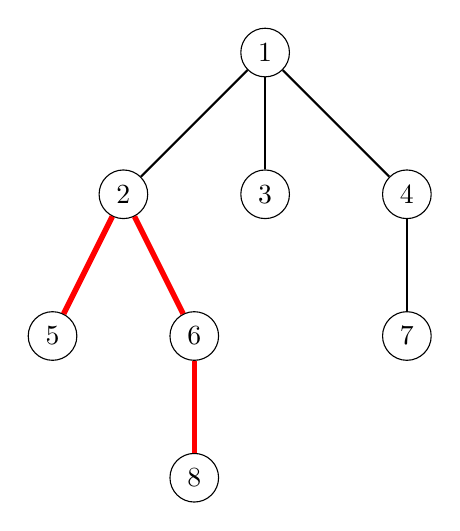
\begin{tikzpicture}[scale=0.9]
\node[draw, circle] (1) at (0,3) {$1$};
\node[draw, circle] (2) at (2,1) {$4$};
\node[draw, circle] (3) at (-2,1) {$2$};
\node[draw, circle] (4) at (0,1) {$3$};
\node[draw, circle] (5) at (2,-1) {$7$};
\node[draw, circle] (6) at (-3,-1) {$5$};
\node[draw, circle] (7) at (-1,-1) {$6$};
\node[draw, circle] (8) at (-1,-3) {$8$};
\path[draw,thick,-] (1) -- (2);
\path[draw,thick,-] (1) -- (3);
\path[draw,thick,-] (1) -- (4);
\path[draw,thick,-] (2) -- (5);
\path[draw,thick,-] (3) -- (6);
\path[draw,thick,-] (3) -- (7);
\path[draw,thick,-] (7) -- (8);

\path[draw=red,thick,-,line width=2pt] (8) -- node[font=\small] {} (7);
\path[draw=red,thick,-,line width=2pt] (7) -- node[font=\small] {} (3);
\path[draw=red,thick,-,line width=2pt] (6) -- node[font=\small] {} (3);
\end{tikzpicture}
\end{center}

5 және 8 төбелерінің жақын арадағы ата-тегі -- 2-төбе.
Төбелердің тереңдігі $\texttt{depth}(5)=3$,
$\texttt{depth}(8)=4$ және $\texttt{depth}(2)=2$ тең.
Сондықтан 5 пен 8 төбелерінің арақашықтығы -- $3+4-2\cdot2=3$.
% The lowest common ancestor of nodes 5 and 8 is node 2.
% The depths of the nodes are
% $\texttt{depth}(5)=3$, $\texttt{depth}(8)=4$ and $\texttt{depth}(2)=2$,
% so the distance between nodes 5 and 8 is
% $3+4-2\cdot2=3$.

\section{Оффлайн алгоритмдер}

Осыған дейін біз тек дарақ сұратымдарына арналған 
\emph{онлайн} алгоритмдер туралы мысалдар келтірдік.
Бұл алгоритмдер сұратымдардың бірінен соң бірін өңдей алады,
яғни әрбір сұратымға келесі сұратымды өңдегенге дейін
жауап береді.
% So far, we have discussed \emph{online} algorithms
% for tree queries.
% Those algorithms are able to process
% queries one after another so that
% each query is answered before receiving the next query.

Дегенмен, көптеген есептер үшін сұратымдарға онлайн жауап
алудың қажеті жоқ.
Осы бөлімде біз \emph{оффлайн} алгоритмдерге мән береміз.
Бұл алгоритмдер сұратымдар жинағына кез келген ретпен жауап береді.
Мұндай алгоритмді қолдану онлайн 
алгоритммен салыстырғанда көбінесе оңайырақ болады.
% However, in many problems, the online
% property is not necessary.
% In this section, we focus on \emph{offline} algorithms.
% Those algorithms are given a set of queries which can
% be answered in any order.
% It is often easier to design an offline algorithm
% compared to an online algorithm.

\subsubsection{Деректер құрылымын біріктіру}

Оффлайн алгоритмді құрудың бір әдісі -- дарақты тереңдігі бойынша
өтіп, төбелерде деректер құрылымын сақтау.
Әр $s$ төбесі үшін оның ұлдарына негізделген $\texttt{d}[s]$ 
деректер құрылымын құрамыз.
Содан соң бұл деректер құрылымын қолдану арқылы біз $s$ төбесіне
байланысты барлық сұратымдарға жауап береміз.
% One method to construct an offline algorithm
% is to perform a depth-first tree traversal
% and maintain data structures in nodes.
% At each node $s$, we create a data structure
% $\texttt{d}[s]$ that is based on the
% data structures of the children of $s$.
% Then, using this data structure,
% all queries related to $s$ are processed.

Мысалға келесі есепті қарастырайық.
Бізге әр төбеге бір мән тағайындалған дарақ беріліп,
''$s$ төбесінің ішдарағына
жататын мәні $x$-ке тең төбелердің санын есептеу''
сұратымдарына жауап беру тапсырылады.
Мысалы, келесі дарақта $4$-төбенің ішдарағында 
мәні 3-ке тең екі төбе бар.
% As an example, consider the following problem:
% % We are given a tree where each node has some value.
% Our task is to process queries of the form
% ''calculate the number of nodes with value $x$
% in the subtree of node $s$''.
% For example, in the following tree,
% the subtree of node $4$ contains two nodes
% whose value is 3.

\begin{center}
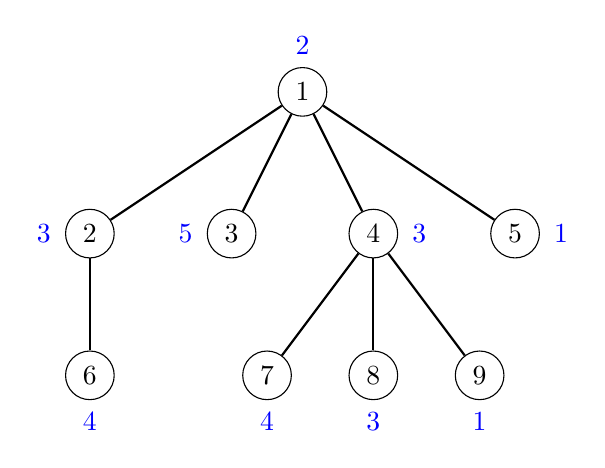
\begin{tikzpicture}[scale=0.9]
\node[draw, circle] (1) at (0,3) {$1$};
\node[draw, circle] (2) at (-3,1) {$2$};
\node[draw, circle] (3) at (-1,1) {$3$};
\node[draw, circle] (4) at (1,1) {$4$};
\node[draw, circle] (5) at (3,1) {$5$};
\node[draw, circle] (6) at (-3,-1) {$6$};
\node[draw, circle] (7) at (-0.5,-1) {$7$};
\node[draw, circle] (8) at (1,-1) {$8$};
\node[draw, circle] (9) at (2.5,-1) {$9$};

\path[draw,thick,-] (1) -- (2);
\path[draw,thick,-] (1) -- (3);
\path[draw,thick,-] (1) -- (4);
\path[draw,thick,-] (1) -- (5);
\path[draw,thick,-] (2) -- (6);
\path[draw,thick,-] (4) -- (7);
\path[draw,thick,-] (4) -- (8);
\path[draw,thick,-] (4) -- (9);

\node[color=blue] at (0,3+0.65) {2};
\node[color=blue] at (-3-0.65,1) {3};
\node[color=blue] at (-1-0.65,1) {5};
\node[color=blue] at (1+0.65,1) {3};
\node[color=blue] at (3+0.65,1) {1};
\node[color=blue] at (-3,-1-0.65) {4};
\node[color=blue] at (-0.5,-1-0.65) {4};
\node[color=blue] at (1,-1-0.65) {3};
\node[color=blue] at (2.5,-1-0.65) {1};
\end{tikzpicture}
\end{center}

Осы есепте сұратымдарға жауап беру 
үшін сөздік құрылымын қолдана аламыз.
Мысалы, 4-төбе және оның ұлдарының сөздігі осылай болмақ
(үстіндегі сан мәнді, ал астындағысы мәннің кездесетін санын
белгілейді):
% In this problem, we can use map structures
% to answer the queries.
% For example, the maps for node 4 and
% its children are as follows:

\begin{center}
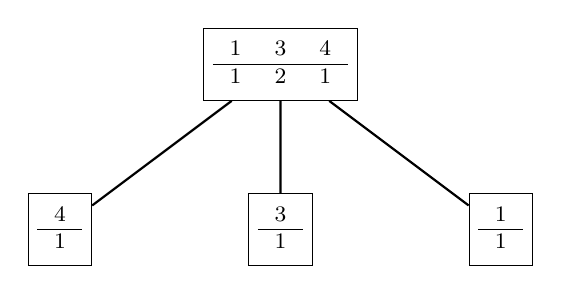
\begin{tikzpicture}[scale=0.7]

\node[draw, rectangle] (a) at (4,5.5)
{
\footnotesize
\begin{tabular}{rrr}
4 \\
\hline
1 \\
\end{tabular}};

\node[draw, rectangle] (b) at (8,5.5)
{
\footnotesize
\begin{tabular}{rrr}
3 \\
\hline
1 \\
\end{tabular}};


\node[draw, rectangle] (c) at (12,5.5)
{
\footnotesize
\begin{tabular}{rr}
1 \\
\hline
1 \\
\end{tabular}};

\node[draw, rectangle] (d) at (8,8.5)
{
\footnotesize
\begin{tabular}{rrr}
1 & 3 & 4 \\
\hline
1 & 2 & 1 \\
\end{tabular}};
\path[draw,thick,-] (a) -- (d);
\path[draw,thick,-] (b) -- (d);
\path[draw,thick,-] (c) -- (d);
\end{tikzpicture}
\end{center}

Егер осындай деректер құрылымын әр төбе үшін құрсақ, біз 
барлық сұратымдарға оңай жауап бере аламыз. Себебі қандай да бір төбеге
байланысты барлық сұратымдарға төбенің деректер құрылымын
құрастырып болғаннан кейін бірден жауап беруге болады.
Мысалы, жоғарыдағы $4$-төбенің сөздік құрылымы бізге 
бұл төбенің ішдарағында мәні 3-ке тең 2 төбе бар екенін 
көрсетеді.
% If we create such a data structure for each node,
% we can easily process all given queries,
% because we can handle all queries related
% to a node immediately after creating its
% data structure. For example, the above
% map structure for node 4
% tells us that its subtree
% contains two nodes whose value is 3.

Дегенмен, барлық деректер құрылымын басынан бастап
құрау тым баяу жүзеге асады.
Оның орнына бастапқыда әр $s$ төбесі үшін тек $s$ төбесінің мәнін сақтайтын  $\texttt{d}[s]$ деректер 
құрылымын құраймыз. Содан соң $s$-тің ұл төбелері арқылы өтіп, $u$ төбесі $s$ -тің ұлы болатын барлық $\texttt{d}[u]$ құрылымын және $\texttt{d}[s]$ -ті қосамыз.
% However, it would be too slow to create
% all data structures from scratch.
% Instead, at each node $s$,
% we create an initial data structure $\texttt{d}[s]$ 
% that only contains the value of $s$.
% After this, we go through the children of $s$ and
% \emph{merge} $\texttt{d}[s]$ and
% all data structures
% $\texttt{d}[u]$ where $u$ is a child of $s$.

Мысалы, жоғарыдағы дарақта $4$-төбенің деректер құрылымы
келесі деректер құрылымдарын біріктіру арқылы шығады:
% For example, in the above tree, the map
% for node $4$ is created by merging the following maps:

\begin{center}
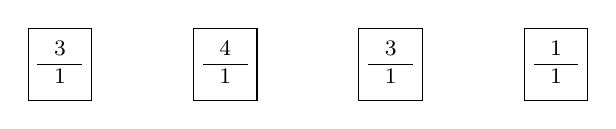
\begin{tikzpicture}[scale=0.7]

\node[draw, rectangle] (a) at (4,5.5)
{
\footnotesize
\begin{tabular}{rrr}
4 \\
\hline
1 \\
\end{tabular}};

\node[draw, rectangle] (b) at (7,5.5)
{
\footnotesize
\begin{tabular}{rrr}
3 \\
\hline
1 \\
\end{tabular}};

\node[draw, rectangle] (c) at (10,5.5)
{
\footnotesize
\begin{tabular}{rr}
1 \\
\hline
1 \\
\end{tabular}};

\node[draw, rectangle] (d) at (1,5.5)
{
\footnotesize
\begin{tabular}{rr}
3 \\
\hline
1 \\
\end{tabular}};

\end{tikzpicture}
\end{center}

Бұл жерде бірінші сөздік $4$-төбенің басындағы деректер
құрылымына және қалған үш сөздік 7, 8 және 9 төбелердің сөздіктеріне сәйкес.
% Here the first map is the initial data structure
% for node 4,
% and the other three maps correspond to nodes 7, 8 and 9.

$s$-төбесінде біріктіру келесі жолмен жүзеге асырылады: $s$ төбесінің барлық ұлдар төбелерін өтіп шығып,
әр $u$ ұл төбесіне $\texttt{d}[u]$ мен 
$\texttt{d}[s]$ -ті қосамыз.
Біз әрдайым $\texttt{d}[u]$ -дің ішіндегісін
$\texttt{d}[s]$ -ке көшіреміз.
Дегенмен $\texttt{d}[s]$
$\texttt{d}[u]$ -ден кіші болса, 
$\texttt{d}[s]$ пен $\texttt{d}[u]$ -дің ішіндегісі алдын ала алмастырылады. Нәтижесінде әрбір мән дарақты айналу процесінде тек $O(\log n)$ рет көшіріледі.
Бұл алгоритмнің тиімділігіне кепілдік береді.
% The merging at node $s$ can be done as follows:
% We go through the children of $s$
% and at each child $u$ merge $\texttt{d}[s]$
% and $\texttt{d}[u]$.
% We always copy the contents from $\texttt{d}[u]$
% to $\texttt{d}[s]$.
% However, before this, we \emph{swap}
% the contents of $\texttt{d}[s]$ and $\texttt{d}[u]$
% if $\texttt{d}[s]$ is smaller than $\texttt{d}[u]$.
% By doing this, each value is copied only $O(\log n)$
% times during the tree traversal,
% which ensures that the algorithm is efficient.

Екі $a$ мен $b$ деректер құрылымын тиімді ауыстыру үшін
біз келесі кодты қолдана аламыз:
% To swap the contents of two data structures $a$ and $b$
% efficiently, we can just use the following code:
\begin{lstlisting}
swap(a,b);
\end{lstlisting}
Егер $a$ мен $b$ C++ тілінің стандартты дерекханасының 
деректер құрылымы болса, жоғарыдағы код тұрақты уақытта жұмыс
істейді.
% It is guaranteed that the above code works in constant time
% when $a$ and $b$ are C++ standard library data structures.

\subsubsection{Жақын арадағы ата-тек}

Сондай-ақ жақын арадағы ата-тектер сұратымдар 
жинағына жауап беретін оффлайн алгоритм бар\footnote{Бұл
алгоритмді Р. Е. Таржан 1979 жылы жариялаған\cite{tar79}.}.
Бұл алгоритм қиылыспайтын жиындар құрылымына негізделген 
(15.2-тарауды еске түсіріңіз). Аталмыш алгоритмнің артықшылығы
-- бөлімде осыған дейін талқыланған алгоритмдерге қарағанда
кодын жазу оңайырақ болуында.

% There is also an offline algorithm
% for processing a set of
% lowest common ancestor queries\footnote{This
% algorithm was published by R. E. Tarjan in 1979 \cite{tar79}.}.
% The algorithm is based on the union-find data structure
% (see Chapter 15.2), and the benefit of the algorithm is
% that it is easier to implement than the
% algorithms discussed earlier in this chapter.

Алгоритмге енгізу ретінде төбелер жұбының жиынтығы
беріледі, ол өз кезегінде әр жұп үшін жақын арадағы ата-текті төбені тауып береді. Алгоритм дарақты тереңдігі бойынша өтіп шығады, оған қоса, төбелердің
қиылыспайтын жиындарын сақтайды.
Бастапқыда әр төбе жеке жиынға жатады.
Әр жиын үшін сол жиынға жататын ең жоғарғы төбені
сақтаймыз.
% The algorithm is given as input a set of pairs of nodes,
% and it determines for each such pair the
% lowest common ancestor of the nodes.
% The algorithm performs a depth-first tree traversal
% and maintains disjoint sets of nodes.
% Initially, each node belongs to a separate set.
% For each set, we also store the highest node in the
% tree that belongs to the set.

Алгоритм $x$ төбесіне жеткенде
$x$ пен $y$ төбелерінің жақын арадағы ата-тегін табуы тиіс барлық 
$y$ төбелерінен өтіп шығады.
Егер $y$ төбесіне әлдеқашан барылған болса, алгоритм
$x$ және $y$ мәндерінің жақын арадағы ата-тегі
$y$ жиынындағы ең жоғарғы төбе екенін хабарлайды.
Кейін $x$ төбені өңдеп болғаннан соң, алгоритм
$x$ жиынын және әкесінің жиынын біріктіреді.
% When the algorithm visits a node $x$,
% it goes through all nodes $y$ such that
% the lowest common ancestor of $x$ and $y$
% has to be found.
% If $y$ has already been visited,
% the algorithm reports that the 
% lowest common ancestor of $x$ and $y$
% is the highest node in the set of $y$.
% Then, after processing node $x$,
% the algorithm joins the sets of $x$ and its parent.

Мысалы, $(5,8)$ және $(2,7)$ төбе жұптарының жақын арадағы ата-тектерін
келесі дарақтан тапқымыз келеді:
% For example, suppose that we want to find the lowest
% common ancestors of node pairs $(5,8)$
% and $(2,7)$ in the following tree:
\begin{center}
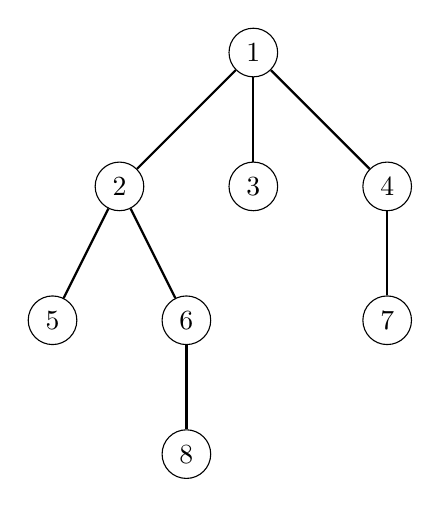
\begin{tikzpicture}[scale=0.85]
\node[draw, circle] (1) at (0,3) {$1$};
\node[draw, circle] (2) at (2,1) {$4$};
\node[draw, circle] (3) at (-2,1) {$2$};
\node[draw, circle] (4) at (0,1) {$3$};
\node[draw, circle] (5) at (2,-1) {$7$};
\node[draw, circle] (6) at (-3,-1) {$5$};
\node[draw, circle] (7) at (-1,-1) {$6$};
\node[draw, circle] (8) at (-1,-3) {$8$};
\path[draw,thick,-] (1) -- (2);
\path[draw,thick,-] (1) -- (3);
\path[draw,thick,-] (1) -- (4);
\path[draw,thick,-] (2) -- (5);
\path[draw,thick,-] (3) -- (6);
\path[draw,thick,-] (3) -- (7);
\path[draw,thick,-] (7) -- (8);\textbf{\textit{}}
\end{tikzpicture}
\end{center}
Төмендегі дарақтардың сұр төбелері барылған төбелерді білдіреді
және төбелердің үзік сызықты топтары бір жиынға жатады.
Алгоритм 8-төбеге жеткенде, ол 5-төбеге барғанын 
және оның жиынындағы ең жоғары төбе 2 екенін байқайды.
Сондықтан 5 және 8 төбелерінің жақын арадағы ата-тегі $2$-төбе болады.
% In the following trees, gray nodes denote visited nodes
% and dashed groups of nodes belong to the same set.
% When the algorithm visits node 8, it notices that
% node 5 has been visited and the highest node
% in its set is 2. Thus, the lowest common ancestor
% of nodes 5 and 8 is 2:
\begin{center}
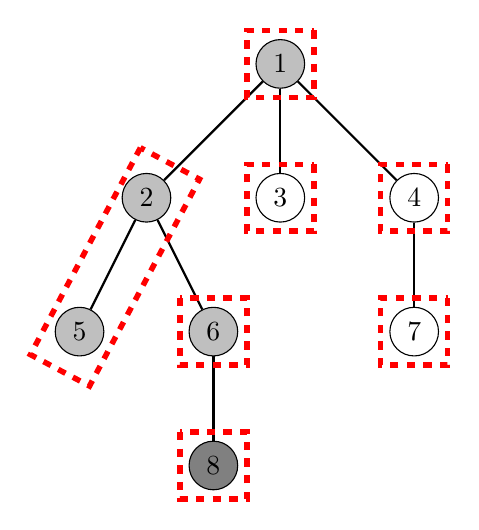
\begin{tikzpicture}[scale=0.85]
\node[draw, circle, fill=lightgray] (1) at (0,3) {$1$};
\node[draw, circle] (2) at (2,1) {$4$};
\node[draw, circle, fill=lightgray] (3) at (-2,1) {$2$};
\node[draw, circle] (4) at (0,1) {$3$};
\node[draw, circle] (5) at (2,-1) {$7$};
\node[draw, circle, fill=lightgray] (6) at (-3,-1) {$5$};
\node[draw, circle, fill=lightgray] (7) at (-1,-1) {$6$};
\node[draw, circle, fill=gray] (8) at (-1,-3) {$8$};
\path[draw,thick,-] (1) -- (2);
\path[draw,thick,-] (1) -- (3);
\path[draw,thick,-] (1) -- (4);
\path[draw,thick,-] (2) -- (5);
\path[draw,thick,-] (3) -- (6);
\path[draw,thick,-] (3) -- (7);
\path[draw,thick,-] (7) -- (8);

\draw [red,thick,dashed,line width=2pt,rotate around={-28:(-2,0)}] (-2.9,1.5) rectangle (-1.9,-2);


\draw [red,thick,dashed,line width=2pt] (-1.5,-0.5) rectangle (-0.5,-1.5);
\draw [red,thick,dashed,line width=2pt] (-1.5,-2.5) rectangle (-0.5,-3.5);

\draw [red,thick,dashed,line width=2pt] (0.5,3.5) rectangle (-0.5,2.5);
\draw [red,thick,dashed,line width=2pt] (0.5,1.5) rectangle (-0.5,0.5);
\draw [red,thick,dashed,line width=2pt] (2.5,1.5) rectangle (1.5,0.5);
\draw [red,thick,dashed,line width=2pt] (2.5,-0.5) rectangle (1.5,-1.5);
\end{tikzpicture}
\end{center}

Алгоритм кейінірек $7$-төбеге барғанда,  
2 мен 7 төбелерінің жақын арадағы ата-тегі болатын $1$-төбені белгілейді.
% Later, when visiting node 7,
% the algorithm determines that
% the lowest common ancestor of nodes 2 and 7 is 1:
\begin{center}
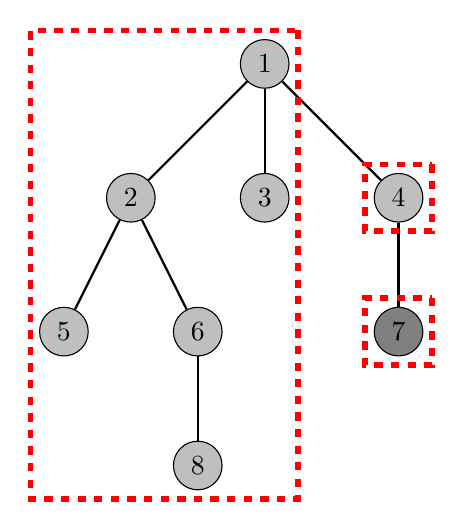
\begin{tikzpicture}[scale=0.85]
\node[draw, circle, fill=lightgray] (1) at (0,3) {$1$};
\node[draw, circle, fill=lightgray] (2) at (2,1) {$4$};
\node[draw, circle, fill=lightgray] (3) at (-2,1) {$2$};
\node[draw, circle, fill=lightgray] (4) at (0,1) {$3$};
\node[draw, circle, fill=gray] (5) at (2,-1) {$7$};
\node[draw, circle, fill=lightgray] (6) at (-3,-1) {$5$};
\node[draw, circle, fill=lightgray] (7) at (-1,-1) {$6$};
\node[draw, circle, fill=lightgray] (8) at (-1,-3) {$8$};
\path[draw,thick,-] (1) -- (2);
\path[draw,thick,-] (1) -- (3);
\path[draw,thick,-] (1) -- (4);
\path[draw,thick,-] (2) -- (5);
\path[draw,thick,-] (3) -- (6);
\path[draw,thick,-] (3) -- (7);
\path[draw,thick,-] (7) -- (8);

\draw [red,thick,dashed,line width=2pt] (0.5,3.5) rectangle (-3.5,-3.5);
\draw [red,thick,dashed,line width=2pt] (2.5,1.5) rectangle (1.5,0.5);
\draw [red,thick,dashed,line width=2pt] (2.5,-0.5) rectangle (1.5,-1.5);

\end{tikzpicture}
\end{center}
